
\section{Selecting Platforms in CLIC}


The platform selection is to find the platform with the lowest cost for each logical operator in the logical plan. 
We take this problem as a node classification problem, where the platform of the lowest cost is considered as the label of the logical operator. 
We use the GCN as the classifier, which is considered more suitable for node classification problems. 
Below we first narrate the feature extraction method used in CLIC and then describe the classification method using GCN.


\subsection{Problem Definition}
In CLIC, a logical plan is organized in the form of DAG. 
We define the DAG as  $G = (V, E)$ where $V$ denotes the logical operator and $E$ denotes the operator dependency.
Our goal is to select the best platform for each logical operator that can achieve the best performance of a workflow. 
We treat the best platform of a logical operator as its label that is decided by the logical plan structure, workload, hardware resources, etc., 
in this way, our goal then becomes classifying a label for each operator in a logical plan, which is a typical node classification problem [].

Such problems with topology as input are usually solved with the Graph Nerual Network(GNN). 
Among many GNNs, the Graph Convolutional Network (GCN) is often used to solve the node classification problems because of its ability to capture neighbor relationships.

\subsection{GCN Intuition}

Graph Convolutional Network is a convolutional neural network that can be directly applied to graphs. 
It applys the convolution kernel to learn the first-order spectral feature, which are followed by activation functions to learn graph representations[42]. 
The convolution kernel learns the spectral feature by inspecting neighboring nodes, below we briefly show the GCN mechanism as an example of the logical plan's node classification process, which is shown in Figure \ref{fig:gcn}.

\begin{figure}
  \centering
  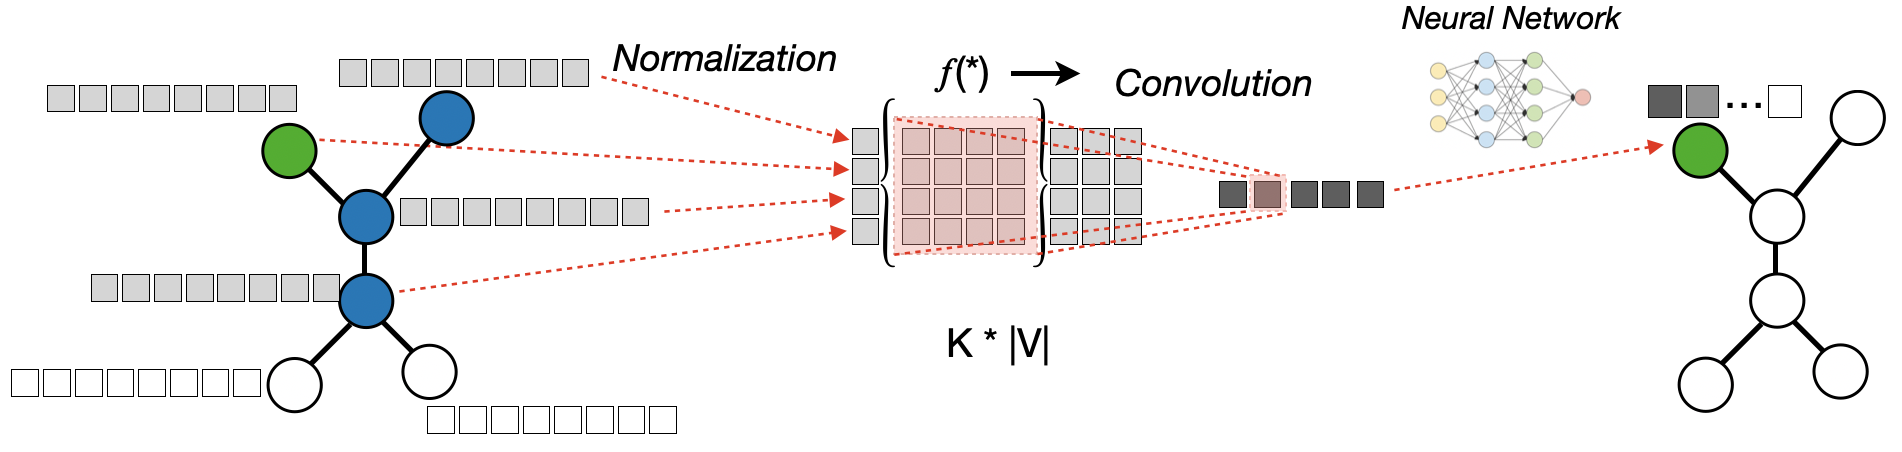
\includegraphics[width=\linewidth]{figures/gcn.png}
  \caption{Selecting platforms with GCN}
  \label{fig:gcn}
\end{figure}

The input of GCN is a graph with nodes are represented as vectors $\hat{V}$. 
In order to learn the relationship between the current operator (green node) and its neighbors, it first needs to normalize the irregular topology to the matrix. 
This is done by selecting the current operator and its K-1 neighbors (blue nodes) to form the K * |V| size matrix. 
Then the kernel function f(x) = AVG(X) slides across the matrix and generates the resulted vector that is the aggregate of its neighborhood. 
After that, the vector is fed into the nerual network to learn the node's graph representation. 
In our classification case, we add a fully-connected layer at the end of the neural network so that the graph representation is transformed into the label's probability distribution immediately. 
Finally, the one with highest probability is selected as the resulted label.

\subsection{Feature Extraction}

As it turns out, many Machine Learning algorithms and almost all Deep Learning Architectures are incapable of processing raw form data like plain text or, in this case, the logical operator. 
They require numbers as inputs to perform any sort of job, be it classification, regression etc. in broad terms. 
Therefore, the operator needs to be vectorized by feature extraction before fed into GCN.

Figure xx shows the structure of few sample operator's feature vector. 
It consists of two segments: the operator encoding and the hardware resources (the right green). 
The following will introduce the meaning of these two segments.

\textbf{Operator Encoding}  
Operators describe the computation logic of the workflow. 
Two logical plan with the same topology can produce radically different classification results due to their different operators. 
Although the first two plans in Figure XX have the same topology, the former is consists of relational operators, which describes the relational algebra over the Table model, and the operators are all classified as the Spark(SQL); 
While the latter describes a linear algebra over the matrix and the operators are all classified as Tensorflow. 
Therefore we use the id to distinguish operators and encode the id using the one-hot encoding. 
The one-hot encoding is used for vectorization of category features, such as gender or id. 
Its vectorization result is a 0-1 vector as shown in Fig.XX (left blue), whose dimension is the same as the number of categories and only has one non-zero element which is the category of the row.


\textbf{Hardware Resources}
Hardware resources, including network bandwidth, GPU memory, SSD/HDD, etc. are also important factors affecting platform classification. 
For example, the selection of two different communication model used in ML frameworks, i.e. the parameter server model and the all-reduce model, are effected by the bandwidth and the GPU. 
In general, the parameter server works better if you have a large number of unreliable and not so powerful machine;
All-reduce works better if you have a small amount of fast devices(variance of step time between each device is small) run in a controlled environment with strong connected links. 
The benchmark result in [ML platform Benchmark] and the experiments in Section 2 also support to this. 
Therefore, we also encode the hardware parameters into the feature vector, as shown in the green segment in Figure xx. 
Those features are the same for all operators in a same plan. 
The Figure xx.3 is the classification result of the same plan with the operator platforms are changed from Tensorflow to PyTorch. 
The reason behind it may be that the network card has been upgraded from 9GBS to 200GBS and the communication model of Tensorflow is set to the parameter server by default, and vice versa for PyTorch. 

\subsection{Training GCN}
The dataset used for training were logical plans and labels of operators in the plan. 
The effectiveness of the model depends on the quality of the dataset. 
Therefore, a large number of logical plans are required first. 
In order to get the labels of each plan, we also need to actually run all of its possible physical plans with different workloads and infrastructures, and choose the one with the least execution time. 
But this confronting two chanllenges: 
i) there lacks sufficient real-world logical plans [] and 
ii) it's impossible to run all the possible physical plans since it is an exponential search space. 

For the former problem, we used the synthesis way to generate the traning data. 
We constructe a state machine for each computing paradigm respectively to represent its programming model, and synthesize the actual logical plans using the markov chain. 

For the latter problem, we first prune the search space using the technique in []. 
And for the last physical plan, we specified the data source and severa; workloads, and run them to get the labels, then we populate the data by interpolation []. 
At last, we repeate the above steps on variational infrastructures.

We train the GCN model using the above synthesized dataset and Figure xx shows the model accuracy on the collected real-world test set. 
It can be seen that, the model acquires pretty good result on the single computing paradigm. 
However, when dealing with the large graph, especially the hybrid graph, the accuracy drops to nearly 50\%, which is unacceptable.

One of the main problem is the one-hot encoding. 
This encoding method always results in a high-dimensional and sparse vector. 
Generally speaking, this makes it less computational since the majority of neural network toolkits do not play well with very high-dimensional, sparse vectors [Neural Network Methods in Natural Language Processing, 2017]. 
The less computational problem is crucial to such a framework since it already faces the insufficiant data problem. 

Another side-effects of the one-hot encoding is that it is imcompatible to a newly integrated operator, which goes against to our high extensible character. 
In particular, the one-hot encoding needs to increase the dimension of all operator vectors whenver a new one is inserted. 
Figure xx examplified this situation where as the new Flatmap operator (red one) being inserted, all the vectors' dimension are grown. 
Thus the previous model needs to be retrained otherwise the new vector becomes an invalid input due to its higher dimension. 
Even if reserving some empty dimension to stablize the input, the model still cannot properly classify the new operator because the new dimension is orthogonal to the other dimension and the model lacks knowledge about this new dimensions.

In order to overcome the above two problems, we turned our attention to represent the operator using the embedding.

\subsection{From One-hot Encoding To Embedding}
In mathmatic, an embedding is a function $f X -> Y$ that maps a data point X in one space to point Y in another space. 
This is the most important preprocess technique in natural language processing (NLP), where the word embedding is a term used for the representation of words for text analysis. 
It is typically in the form of a real-valued vector that encodes the meaning of the word such that the words that are closer in the vector space are expected to be similar in meaning [wiki]. 
For promotion, there also are image embedding, video embedding. 
A representative algorithm for generating word embedding is the CBOW[], whose main idea is that words appearing in the same sentence have higher relevance. 
The way CBOW works, in a nutshell, is that it tends to maximize the joint probability of a word and its context words in a sentence. 
Therefore, its training requires a large corpus containing enough sentences.

We can share the same idea in the word embedding that allows semantically similar operators to have closer distance. 
The objective function is the also the same when training the operator embedding, i.e. maximizing the joint probability of a operator and its neighbor operators in a logical plan, therefore we can still use the CBOW algorithm. 
We take a logical plan as a "sentence", where each operator is a "word" and the "context words" are the remaining operators in the logical plan. 
All we need to do is provide a number of logical plans as the corpus. 
Fortunately, we already have a large number of synthetic logical plans. 
The resulting embeddings are shown in Figure xx. 
For the sake of visualization, we just show the top-2 dimensions with the highest eigenvalue. 
One observation is that operators that are the same computing paradigm and have the same number of inputs and outputs tend to have small cosine distance. 
What's more, the newly inserted Flatmap operator is mapped closer to the Map operator instead of the Matmul operator which is probably due to the same reason. 
In another word, the operator embedding now has some semantic meanings.

After replacing the one-hot encoding to the operator embedding, we overcome the above two problem: 
\begin{itemize}
    \item 1) The operator embedding is low-dimensional and dense compare to the one-hot encoding, which means more computational. 
    As shown in Figure xx, the classification accuracy increased significantly especially for the large graph. 
    \item 2) It's now compatible to a newly integrated operator. 
    Figure xx outlines the embedding structure of both the old and new operator. 
    It can be seen that, both the two types of operator have the same dimension and are in the same euclidean space, therefore the new operator not only does not cause dimensional changes and ultimately invalidate the model, but because the embedding represents a certain semantic relationship, the model can make the inference for it directly using the existing knowledge. 
\end{itemize}

There are two scenario for getting the embedding of a new operator:
\begin{itemize}
    \item 1) The operator is new to CLIC but not the model, therefore its embedding can be retreived in CLIC directly from the model.
    \item 2) The operator is also new to the model, i.e. the "OOV" (out of vocabulary) problem. 
    In this case, the model needs some new training data to recognize it. 
    Therefore, we synthesize some new logical plan that contains the operator according to operator's attributes and then incrementally updates the model to generate the embedding.
\end{itemize}

Apart from the above operator embedding, we also design and generate the embedding for each physical computing platform. 
The main motivation for this is the compatibility: a newly supported platform will increase the number of categories to predict which will also invalidate the model. 
But with the platform embedding, we can change the classification policy from "selecting the one with highest probability" to "selecting the closest one to the resulting embedding". 
The mathmatical meaning and generation method goes the same. 
The only difference is that instead of treating the operator as the "word", we treat each platform that supports the operator as the "word". 
The resulting Platform Embedding is shown in Figure XX.

Last but not the least, it's important to emphasize that both the operator and platform embedding techniques are not neccessarily bound with CLIC but a general feature extraction method. 
One can generate an operator embedding whether the operator is supported by CLIC or not as long as there are logical plans that contain this operator.

% \begin{figure}
%     \subfigure[One-Hot Encoding]{
%         \label{fig:one-hot}
%         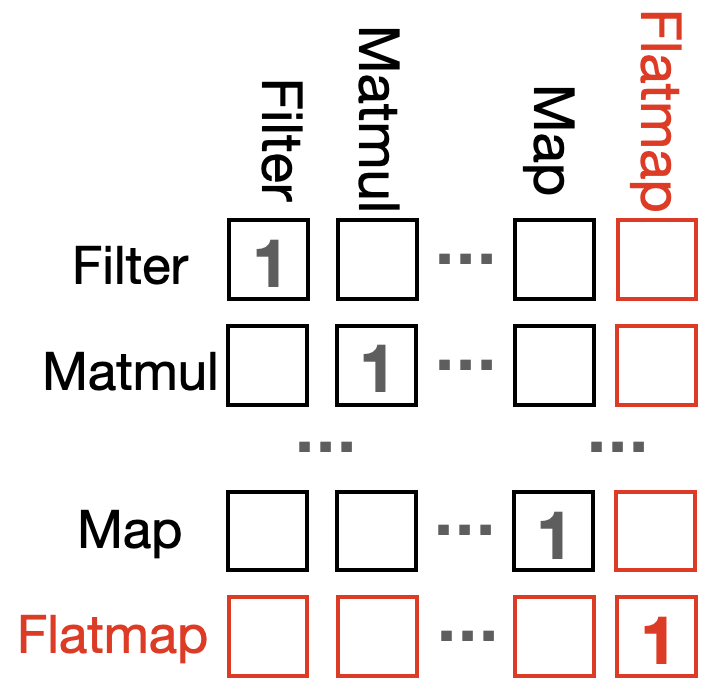
\includegraphics[width=0.3\linewidth]{figures/one-hot.png}
%     } 
%     \subfigure[Operator Embedding]{
%         \label{fig:embedding}
%         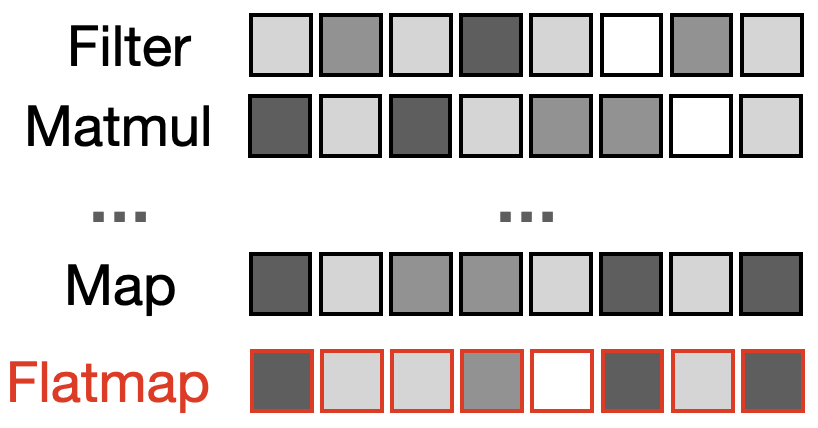
\includegraphics[width=0.3\linewidth]{figures/embedding.png}
%     } 
%     \caption{Vectoization Method}
%     \label{fig:encoding}
% \end{figure}


% \subsection{Data Generation}
% \textbf{Generating Operator Embedding}
% In word embedding, because the words in a sentence have certain correlation with its context words, 
% the cost function of training Word Embedding is to maximum the joint probability of the word and its context words. 
% Similarly, we can also reasonably assume that the operators that appear in a same logical plan have certain correlation and use the same cost function. 
% We take the topological-ordered logical plan as the sentence and the logical operators inside are words, 
% then use the same model to train the operator embedding. The results are shown in Figure xx. 
% For the sake of visualization, we just show the top-2 dimensions with the highest eigenvalue. 
% One observation is that operators that are the same computing paradigm and have the same number of inputs and outputs tend to have small cosine distance. 
% What's more, the newly inserted Flatmap operator is also mapped closer to the Map operator instead of the Matmul operator which is probably due to the same reason.

% % TODO: 图之后再调整
% \begin{figure}
%     \subfigure[Operator Embedding]{
%         \label{fig:opt_ebd}
%         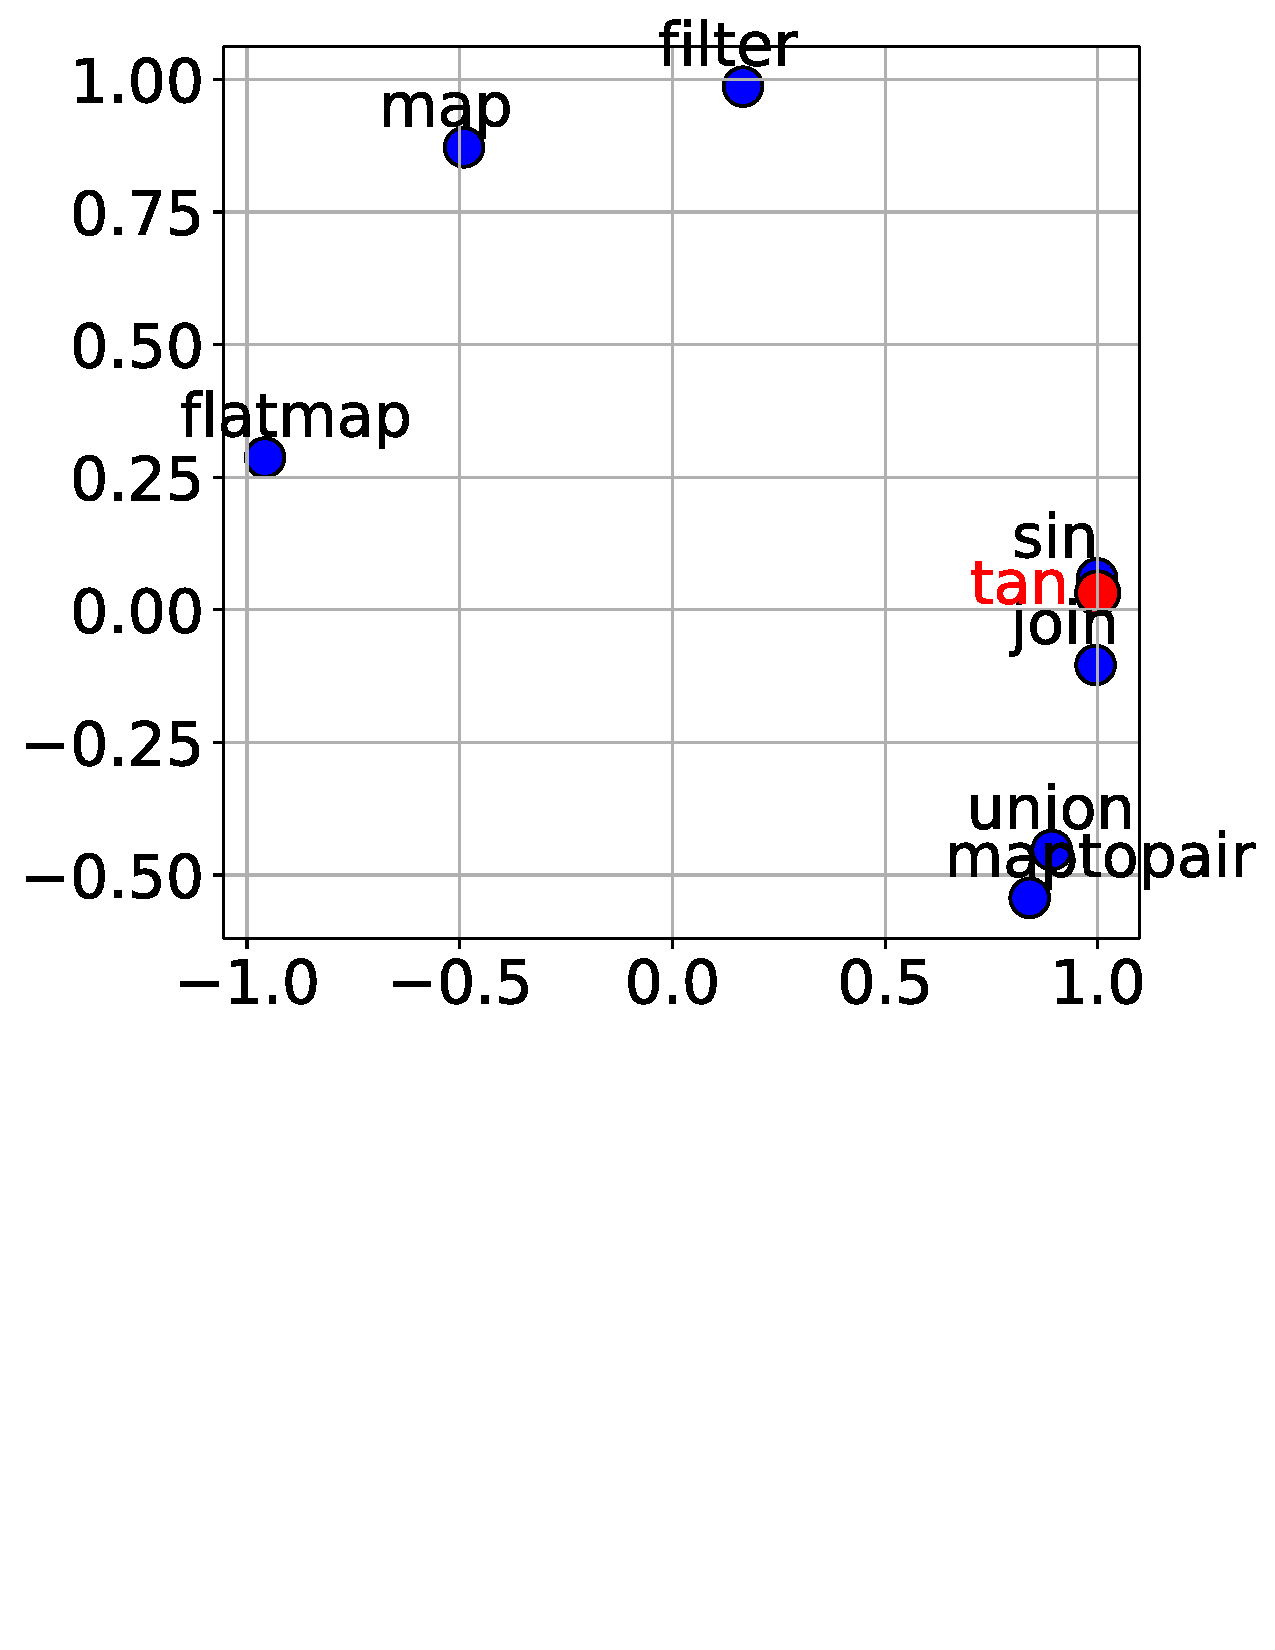
\includegraphics[width=0.4\linewidth]{figures/embedding_visual.pdf}
%     } 
%     \subfigure[Platform Embedding]{
%         \label{fig:embedding}
%         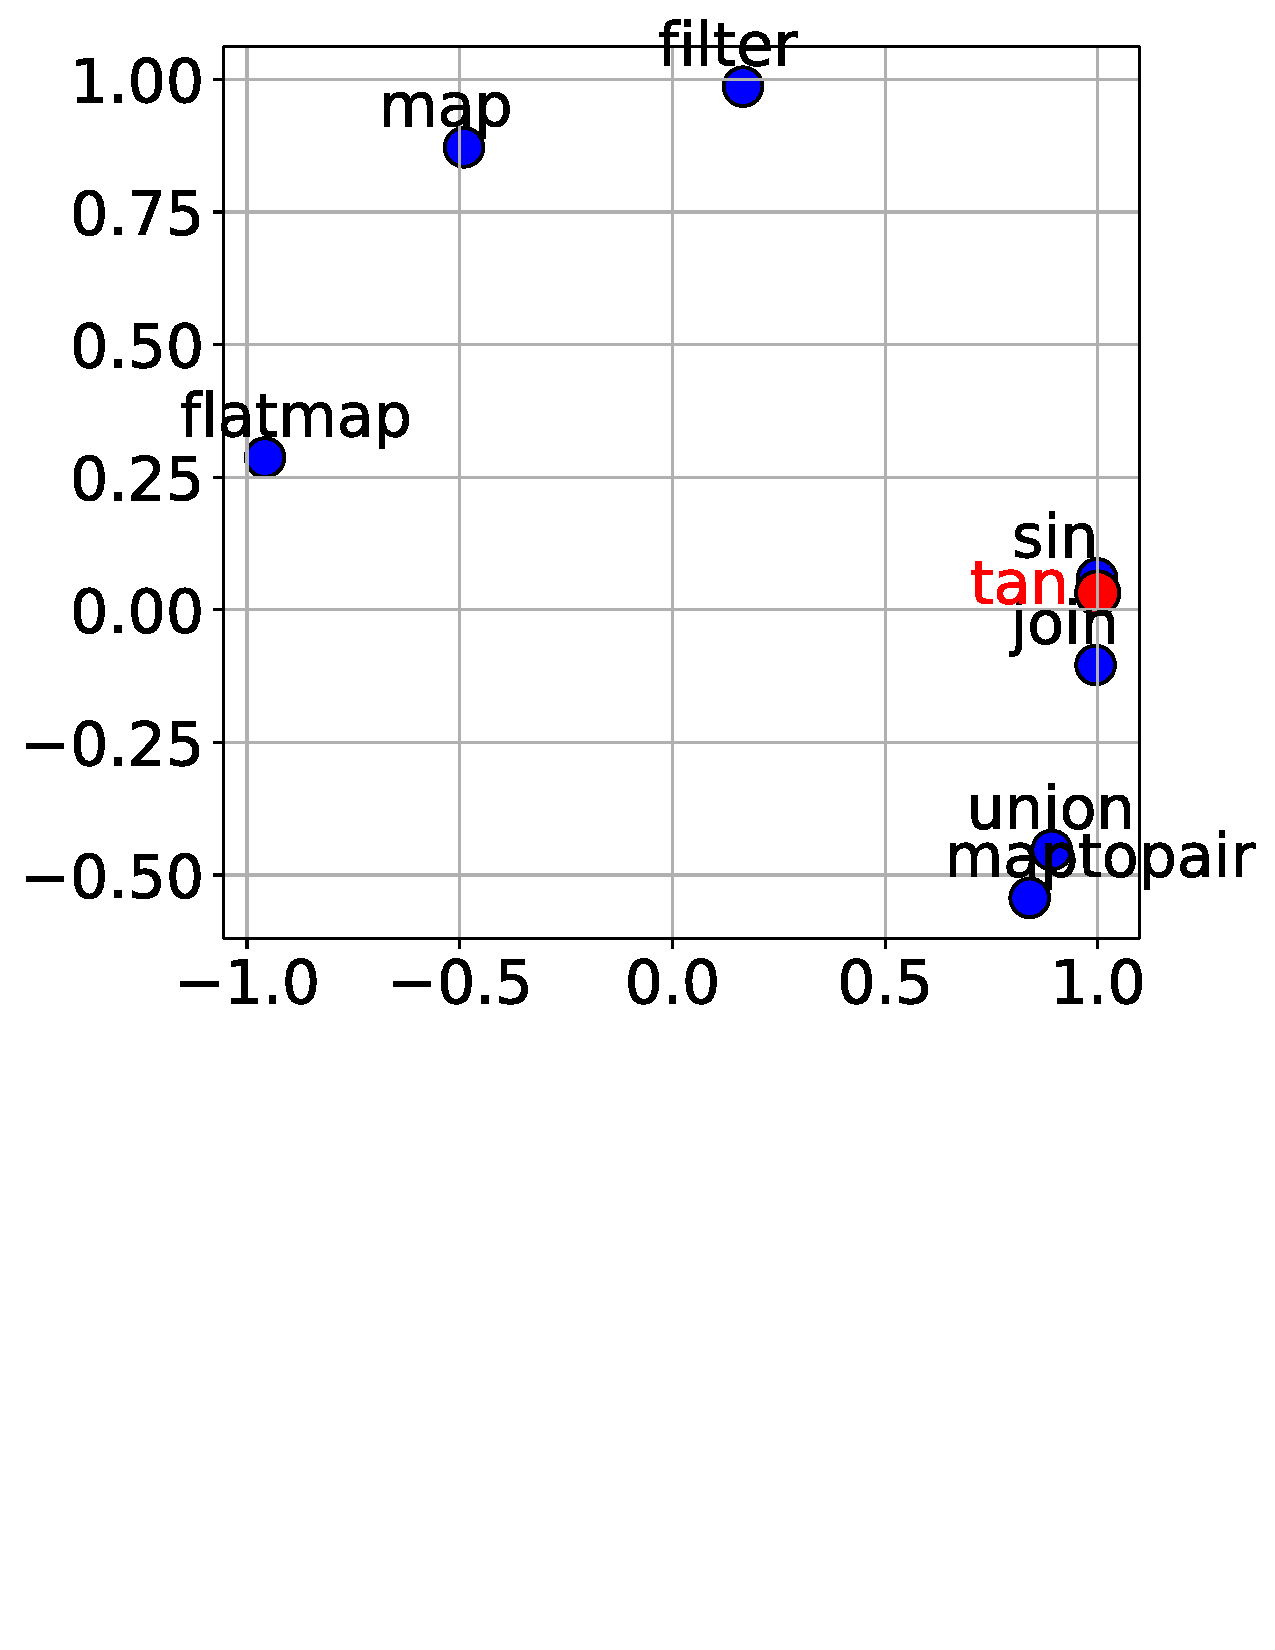
\includegraphics[width=0.4\linewidth]{figures/embedding_visual.pdf}
%     } 
%     \caption{Embedding Visualization}
%     \label{fig:embedding_panel}
% \end{figure}

% It's important to emphasize that the operator embedding technique is not bound with CLIC but a general feature extraction method. 
% One can generate an operator embedding whether the operator is supported by CLIC or not as long as there are logical plans that contain this operator.

% As we have mentioned that the operator embedding is compatible for the newly integrated operator. 
% There're two cases when integrating a new operator:
% \begin{itemize}
%     \item [1)]
%     The operator is new to CLIC but not the model, therefore its embedding can be retreived in CLIC directly from the model.
%     \item [2)]
%     The operator is also new to the model, i.e. the "OOV" (out of vocabulary) problem. 
%     In this case, the model needs some new training data to recognize it. 
%     Therefore, we synthesize some new logical plan that contains the operator according to operator's attributes and then incrementally updates the model to generate the embedding.
% \end{itemize}

% Apart from the above operator embedding, 
% we also design and generate the embedding for each physical computing platform. 
% The mathmatical meaning and generation method goes the same. 
% We don't further explain due to limits of space.


% \textbf{Generating Training Data}
% The effectiveness of the GCN strongly depends on the training data. 
% In our case, a large amount of disparate logical plans (data points) together with the best physical platform (labels) of each logical operator in it is required. 
% The logical operator's feature vector is composed of two parts: operator embedding and the global hardware resources. 
% % 1. 举例子说明为什么考虑带宽
% % 2. 把向量图画出来
% % 3. 把这段提前
% The latter is the same for the operators in the same logical plan, including infrastructure's CPU frequency, main memory, GPU memory, network bandwidth, etc. 
% However, there is currently a lack of the Workflow dataset for cross-platform computation, so we borrow the TDGen [] to synthesized datasets separately for each computation mode and on different infrastructures.